\documentclass[12pt]{book}
\usepackage{fontspec}
\setmainfont{TeX Gyre Pagella}
\usepackage[paperwidth=8in,paperheight=8in,margin=0.6in]{geometry}
\usepackage{xcolor}
\usepackage{tikz}
\usepackage{graphicx}
\pagestyle{empty}
\setlength{\parindent}{0pt}

\newcommand{\artnote}[1]{{\color{gray!70}\small\itshape [Illustration: #1]}\par\vspace{0.3in}}
\newcommand{\bigline}[1]{{\Huge #1}\par}
\newcommand{\pagenum}[1]{\vfill{\color{gray!50}\footnotesize #1}}
\newcommand{\sprollpage}{\newpage\vspace*{0.4in}}

\begin{document}

% ============ FRONT COVER ============
\thispagestyle{empty}
\begin{center}
\vspace*{1.2in}
{\Huge \textbf{SPROLL 01}}\\[0.4in]
{\huge \textbf{One Pop}}\\[0.6in]
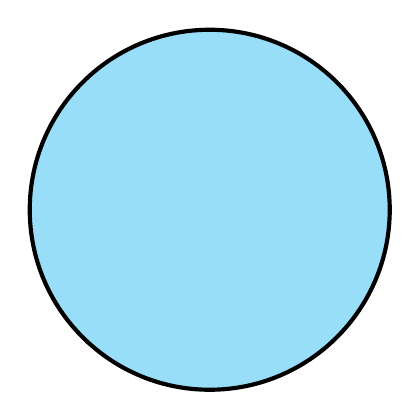
\begin{tikzpicture}
\filldraw[fill=cyan!40,draw=black,line width=1.5pt] (0,0) circle (0.9in);
\end{tikzpicture}\\[0.6in]
{\large \textit{a first book of distinctions}}\\[0.3in]
{\small The Sproll Curriculum $\cdot$ Cycle I: Pops}
\end{center}

% ============ PAGE 2: half-title / indicia ============
\sprollpage
\begin{center}
\vspace*{1.5in}
{\Large The Sproll Curriculum}\\[0.2in]
{\normalsize Cycle I --- Pops: Things, Differences, and Counting}\\[0.6in]
{\small Sproll 01 of 40}
\end{center}
\pagenum{2}

% ============ PAGE 3 ============
\sprollpage
\begin{center}
\vspace*{0.6in}
\artnote{a single small solid dot, alone in the center of an otherwise empty page}
\bigline{Here is a Pop.}
\vspace{0.3in}

\begin{tikzpicture}
\filldraw[fill=black] (0,0) circle (0.15in);
\end{tikzpicture}
\vspace{0.3in}
\bigline{We noticed something.}
\end{center}
\pagenum{3}

% ============ PAGE 4 ============
\sprollpage
\begin{center}
\vspace*{0.6in}
\artnote{a red scribble-mark, roughly circular but hand-drawn and irregular}

\begin{tikzpicture}
\draw[red, line width=3pt] plot [smooth cycle] coordinates {(0,0.3) (0.3,0.5) (0.5,0.1) (0.2,-0.3) (-0.3,-0.1) (-0.2,0.2)};
\end{tikzpicture}
\vspace{0.4in}
\bigline{A red mark can Pop.}
\end{center}
\pagenum{4}

% ============ PAGE 5 ============
\sprollpage
\begin{center}
\vspace*{0.6in}
\artnote{a simple drawn sound-wave burst, or a child clapping with small motion lines around the hands}
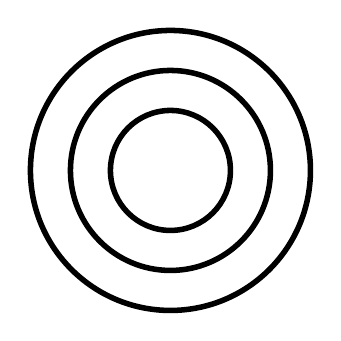
\begin{tikzpicture}
\draw[line width=2pt] (0,0) circle (0.3in);
\draw[line width=2pt] (0,0) circle (0.5in);
\draw[line width=2pt] (0,0) circle (0.7in);
\end{tikzpicture}
\vspace{0.4in}
\bigline{A sound can Pop.}
\end{center}
\pagenum{5}

% ============ PAGE 6 ============
\sprollpage
\begin{center}
\vspace*{0.6in}
\artnote{two hands mid-clap, simple line drawing, small motion marks between the palms}

\begin{tikzpicture}
\draw[line width=2pt] (-0.4,0) -- (-0.05,0.1);
\draw[line width=2pt] (0.4,0) -- (0.05,0.1);
\draw[line width=1pt] (0,0.15) -- (0,0.4);
\draw[line width=1pt] (-0.15,0.2) -- (-0.3,0.45);
\draw[line width=1pt] (0.15,0.2) -- (0.3,0.45);
\end{tikzpicture}
\vspace{0.4in}
\bigline{A clap can Pop.}
\end{center}
\pagenum{6}

% ============ PAGE 7 ============
\sprollpage
\begin{center}
\vspace*{0.6in}
\artnote{a simple black square outline, evenly drawn}

\begin{tikzpicture}
\draw[line width=3pt] (-0.4,-0.4) rectangle (0.4,0.4);
\end{tikzpicture}
\vspace{0.4in}
\bigline{A square can Pop.}
\end{center}
\pagenum{7}

% ============ PAGE 8 ============
\sprollpage
\begin{center}
\vspace*{0.6in}
\artnote{a large, dense, tangled scribble filling most of the space, deliberately messy and complicated}
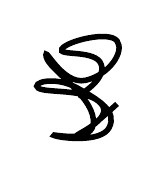
\begin{tikzpicture}
\draw[line width=2pt] plot [smooth, tension=1.2] coordinates
{(0,0) (0.3,0.4) (-0.2,0.6) (0.5,0.7) (0.1,0.2) (-0.4,0.5) (0.2,-0.3)
(-0.3,-0.5) (0.4,-0.4) (0,0.1) (-0.5,0.1) (0.3,-0.1) (0,-0.5) (0.5,-0.1)};
\end{tikzpicture}
\vspace{0.4in}
\bigline{A large, complicated scribble can Pop.}
\end{center}
\pagenum{8}

% ============ PAGE 9 ============
\sprollpage
\begin{center}
\vspace*{0.6in}
\artnote{no new image; small versions of the dot, mark, square, and scribble arranged in a loose row, all equal in size}

\begin{tikzpicture}
\filldraw[fill=black] (-1.4,0) circle (0.12in);
\draw[red, line width=2pt] plot [smooth cycle] coordinates {(-0.5,0.15) (-0.35,0.25) (-0.25,0.05) (-0.4,-0.1) (-0.55,-0.05)};
\draw[line width=2pt] (0.15,-0.13) rectangle (0.45,0.13);
\draw[line width=1.5pt] plot [smooth, tension=1.2] coordinates
{(0.9,0) (1.0,0.15) (0.85,0.2) (1.05,0.05) (0.95,-0.1) (1.1,-0.05)};
\end{tikzpicture}
\vspace{0.4in}
\bigline{Pop does not mean dot.}\vspace{0.1in}
\bigline{Pop does not mean circle.}\vspace{0.1in}
\bigline{Pop does not mean number.}\vspace{0.2in}
{\Huge \textbf{Pop means: something we noticed.}}
\end{center}
\pagenum{9}

% ============ PAGE 10 ============
\sprollpage
\begin{center}
\vspace*{0.6in}
\artnote{two identical small dots side by side, same size, same color}
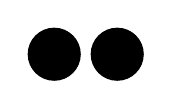
\begin{tikzpicture}
\filldraw[fill=black] (-0.4,0) circle (0.13in);
\filldraw[fill=black] (0.4,0) circle (0.13in);
\end{tikzpicture}
\vspace{0.4in}
\bigline{How many Pops?}
\end{center}
\pagenum{10}

% ============ PAGE 11 ============
\sprollpage
\begin{center}
\vspace*{0.4in}
\artnote{two identical small dots, but this time placed far apart -- one near the top left of the page, one near the bottom right}
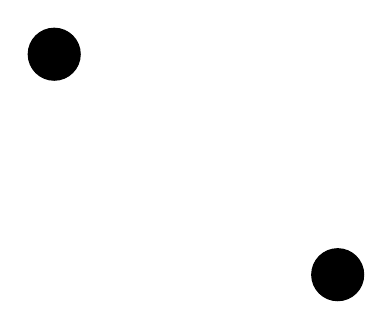
\begin{tikzpicture}[remember picture]
\filldraw[fill=black] (-1.8,1.4) circle (0.13in);
\filldraw[fill=black] (1.8,-1.4) circle (0.13in);
\end{tikzpicture}
\vspace{2.2in}
\bigline{Are these the same Pop?}
\end{center}
\pagenum{11}

% ============ PAGE 12 ============
\sprollpage
\begin{center}
\vspace*{0.6in}
\artnote{the same two dots from the previous page, now shown together in one small frame, still in their separate positions, with a faint dotted line connecting them}
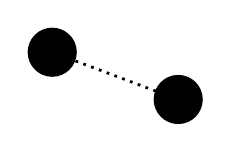
\begin{tikzpicture}
\filldraw[fill=black] (-0.8,0.3) circle (0.12in);
\filldraw[fill=black] (0.8,-0.3) circle (0.12in);
\draw[dotted, line width=1pt] (-0.8,0.3) -- (0.8,-0.3);
\end{tikzpicture}
\vspace{0.4in}
\bigline{They look the same.}\vspace{0.15in}
\bigline{But one is here.}\vspace{0.15in}
\bigline{And one is there.}
\end{center}
\pagenum{12}

% ============ PAGE 13 ============
\sprollpage
\begin{center}
\vspace*{0.5in}
\artnote{a large circular boundary containing a small busy scene inside it: a few dots, a mark, a small shape, all clustered together, with the boundary drawn clearly around the whole group}
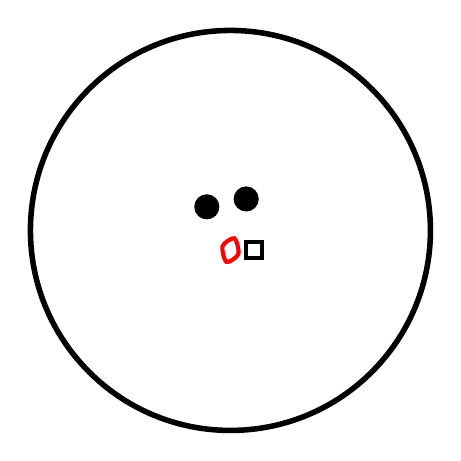
\begin{tikzpicture}
\draw[line width=2pt] (0,0) circle (1in);
\filldraw[fill=black] (-0.3,0.3) circle (0.06in);
\filldraw[fill=black] (0.2,0.4) circle (0.06in);
\draw[red, line width=1.5pt] plot [smooth cycle] coordinates {(-0.1,-0.2) (0.05,-0.1) (0.1,-0.3) (-0.05,-0.4)};
\draw[line width=1.5pt] (0.2,-0.35) rectangle (0.4,-0.15);
\end{tikzpicture}
\vspace{0.4in}
\bigline{Can the whole thing Pop?}
\end{center}
\pagenum{13}

% ============ PAGE 14 ============
\sprollpage
\begin{center}
\vspace*{0.5in}
\artnote{the same circular scene from the previous page, but now drawn as a single solid dot the same size as the very first Pop on page 3, with the small boundary circle still faintly visible around it}

\begin{tikzpicture}
\draw[line width=1pt, gray!50] (0,0) circle (0.5in);
\filldraw[fill=black] (0,0) circle (0.18in);
\end{tikzpicture}
\vspace{0.4in}
\bigline{Yes.}\vspace{0.15in}
{\Large A Pop can be one thing.}\\[0.1in]
{\Large A Pop can also be many things,}\\[0.1in]
{\Large held together as one.}
\end{center}
\pagenum{14}

% ============ PAGE 15 (closing / hand-off) ============
\sprollpage
\begin{center}
\vspace*{0.5in}
\artnote{one solid dot on the left, one solid triangle on the right, with visible empty space between them}

\begin{tikzpicture}
\filldraw[fill=black] (-0.9,0) circle (0.15in);
\draw[fill=black] (0.7,-0.25) -- (0.9,0.25) -- (1.1,-0.25) -- cycle;
\end{tikzpicture}
\vspace{0.4in}
\bigline{One Pop. Another Pop.}\vspace{0.3in}
{\Large What could happen between them?}
\vspace{0.5in}\\
{\small \textit{--- turn the page for Sproll 02: Another Pop ---}}
\end{center}
\pagenum{15}

% ============ PAGE 16: Note for Grown-Ups (backmatter) ============
\sprollpage
\vspace*{0.3in}
{\large \textbf{A Note for Grown-Ups}}
\vspace{0.2in}

\normalsize
This book teaches no arithmetic and asks for no answers. Its only goal is to let a child practice the single act underneath all of mathematics: noticing that something can be told apart from everything around it. We call that a Pop.

\vspace{0.15in}
Nothing in this book is ever calculated. That is deliberate. Sproll 01 is not withholding arithmetic out of caution; it is establishing that mathematics begins earlier than arithmetic does, in the ordinary act of distinguishing one thing from its surroundings.

\vspace{0.15in}
The two open questions in this book, ``Are these the same Pop?'' and ``Can the whole thing Pop?'', are not meant to be answered for the child. Sitting with them is the point. Later Sprolls return to both questions with more to say.

\vspace{0.15in}
There is no need to introduce the word ``Pop'' as a technical term, a formula, or a rule. It only needs to mean, for now, ``something we noticed.''

\vspace{0.3in}
{\small Sproll 02: Another Pop continues directly from this book's final page.}
\pagenum{16}

\end{document}
